\documentclass[12pt]{article}
\usepackage[left=1in,right=1in,top=1in,bottom=1in]{geometry}
\usepackage[utf8]{inputenc}
\usepackage{graphicx}
\usepackage{pdflscape}
\usepackage{float}
\usepackage{geometry}
\usepackage{hyperref}
\usepackage{indentfirst}
\usepackage[justification=centering,labelfont=bf]{caption}
\usepackage{amsmath, amsfonts, amssymb, amsthm}

\title{
\includegraphics[height=3cm]{pics/UVM.png} \\
    CS352 Evolutionary Computation: Homework 4}
\author{Ayat Ospanov}
\date{\today}

\begin{document}

\maketitle

\section{Experiments}\label{sec:experiments}

    The experiment was conducted to explore the capabilities of genetic programming
    using Eureqa. For the experiment, there was constructed the next function:
    $$f(x, y) = \frac{x}{\log(y)} + \sin(x)e^y$$

    The ``formula building-blocks'' for Eureqa were: a constant, a variable,
    addition and subtraction operators, multiplication and division operators,
    sine and cosine, exponential, natural logarithm and power operators. The
    data for the experiment were generated uniformly in amount of 100 for the
    next ranges of the arguments:
    \begin{align*}
        x &\in [-5, 5] \\
        y &\in [1.1, 5.1]
    \end{align*}

    The experiment was done on noisy data with different amplitude of noise added
    to function values and the arguments. All noises added were Gaussian noise
    with mean of 0 and standard deviation of $\sigma \in \{0.5, 2.5, 5\}$ for the
    values of the function, and $\sigma = 0.5$ for the values of the function
    with $\sigma_x = 0.05, \sigma_y = 0.02$ for the arguments $x$ and $y$ respectively.

    \begin{figure}[H]
        \centering
        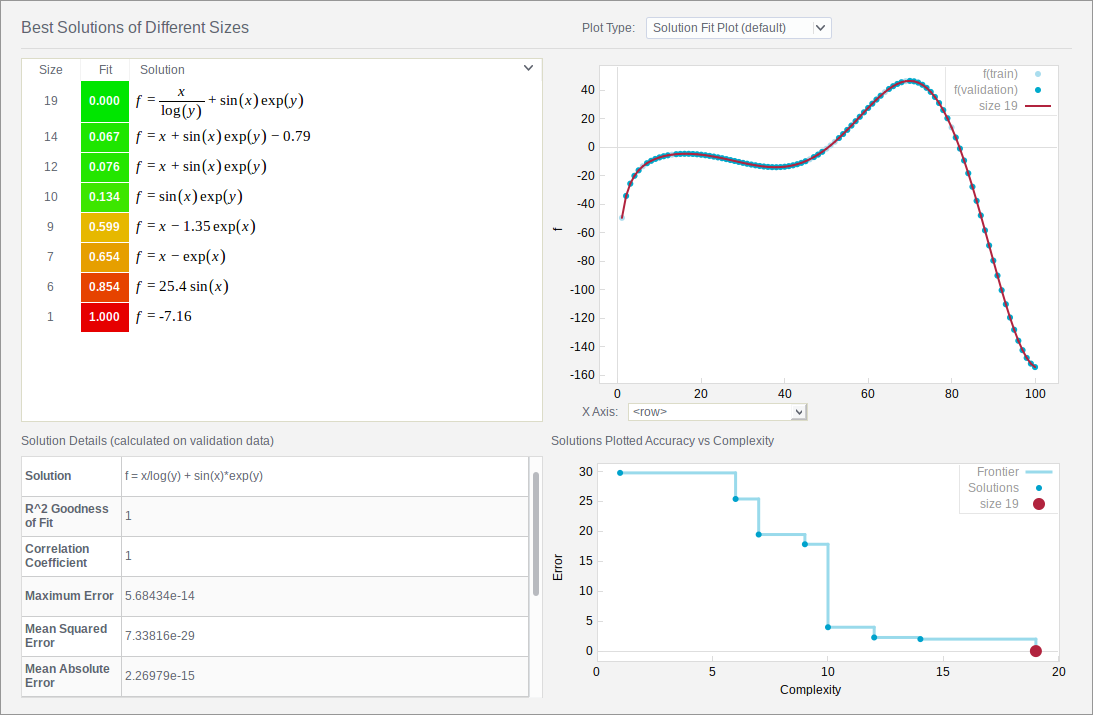
\includegraphics[width=\linewidth]{pics/sol_0.png}
        \caption{Run on the original data}
        \label{fig:noiseless}
    \end{figure}

    Before beginning the experiment, let's check if Eureqa can find our function
    using the original noiseless data. As it is shown on \autoref{fig:noiseless},
    Eureqa were able to find the exact solution. The solution lays on the point
    where Error is 0 on the front for Error vs. Complexity plane. It is obvious
    that if we have an error of 0 on validation data, then we found the solution
    and for reasonable complexity it is the best solution.

    \begin{figure}[H]
        \centering
        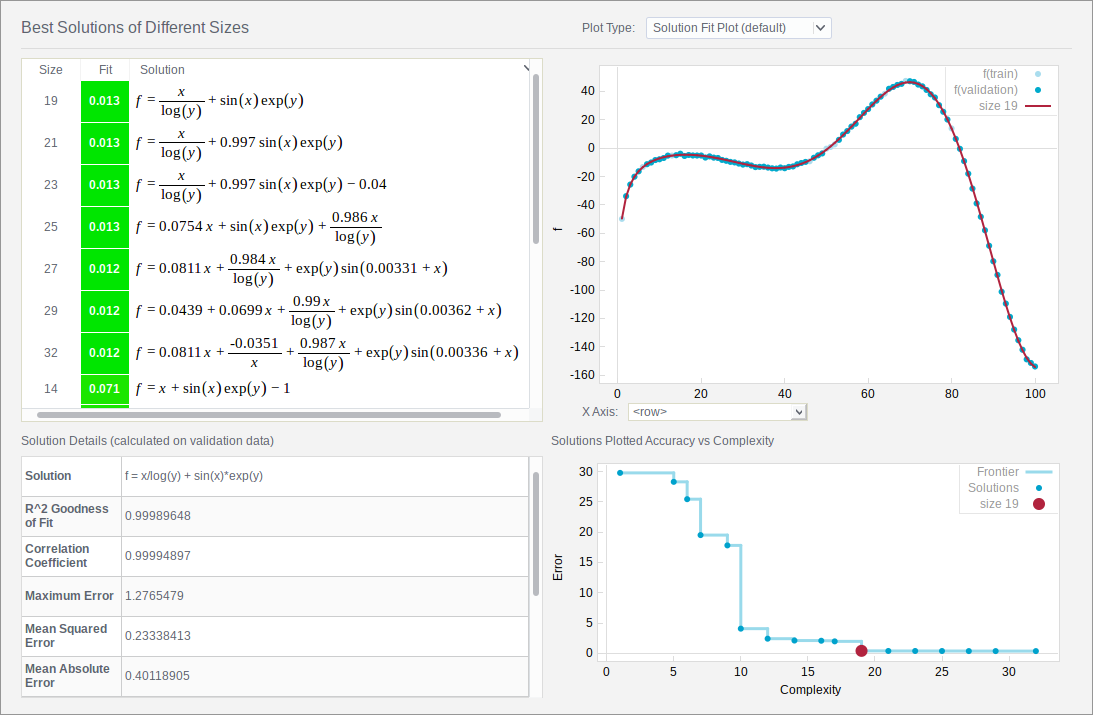
\includegraphics[width=\linewidth]{pics/sol_1perc.png}
        \caption{Run on the noisy function values with $\sigma = 0.5$}
        \label{fig:s_05}
    \end{figure}

    As we made sure that our function can be built by Eureqa from the data, let's
    try to add some noise to the function values and look if Eureqa can find the
    solution.

    First, try to add noise of 1\% of function values' standard deviation (std)
    and run the program. As the function values' std is about 50, then $\sigma=0.5$.

    Adding little noise did not prevent GP algorithms from finding the exact solution
    (\autoref{fig:s_05}). As there is some noise in our data, we have more than
    one close to each other solutions. For example:
    $$f(x, y) = \frac{x}{\log(y)} + 0.997\sin(x)e^y - 0.04$$

    These solutions have approximately equal errors on validation data, but Eureqa
    chose the less complex one which is our function.

    \begin{figure}[H]
        \centering
        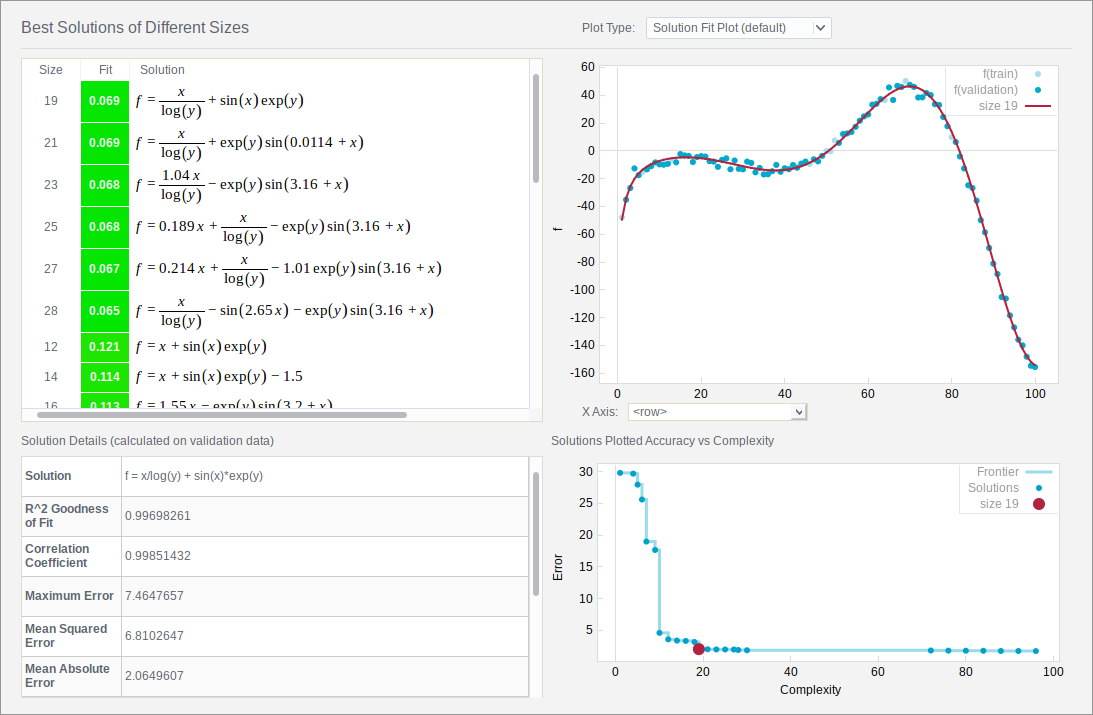
\includegraphics[width=\linewidth]{pics/sol_5perc.png}
        \caption{Run on the noisy function values with $\sigma = 2.5$}
        \label{fig:s_25}
    \end{figure}

    Now let's test the program for the values with more noise. Say, our function
    values have the error of measurement of 5\%. This is $\sigma = 2.5$. As it
    can be seen on the plot in \autoref{fig:s_25}, it is enough to ``shake'' our
    data. Even we added more noise, Eureqa was possible to find the exact solution.
    As in the previous test, we have several close to each other solutions. The
    interesting one is
    $$f(x, y) = \frac{1.04x}{\log(y)} - e^y\sin(3.16 + x)$$

    As we know from trigonometry, $sin(\pi + x) = -sin(x)$. And as $3.16 \approx
    \pi$, this result is really interesting. Here again Eureqa chose the less
    complex one while keeping Error almost at the minimum.

    \begin{figure}[H]
        \centering
        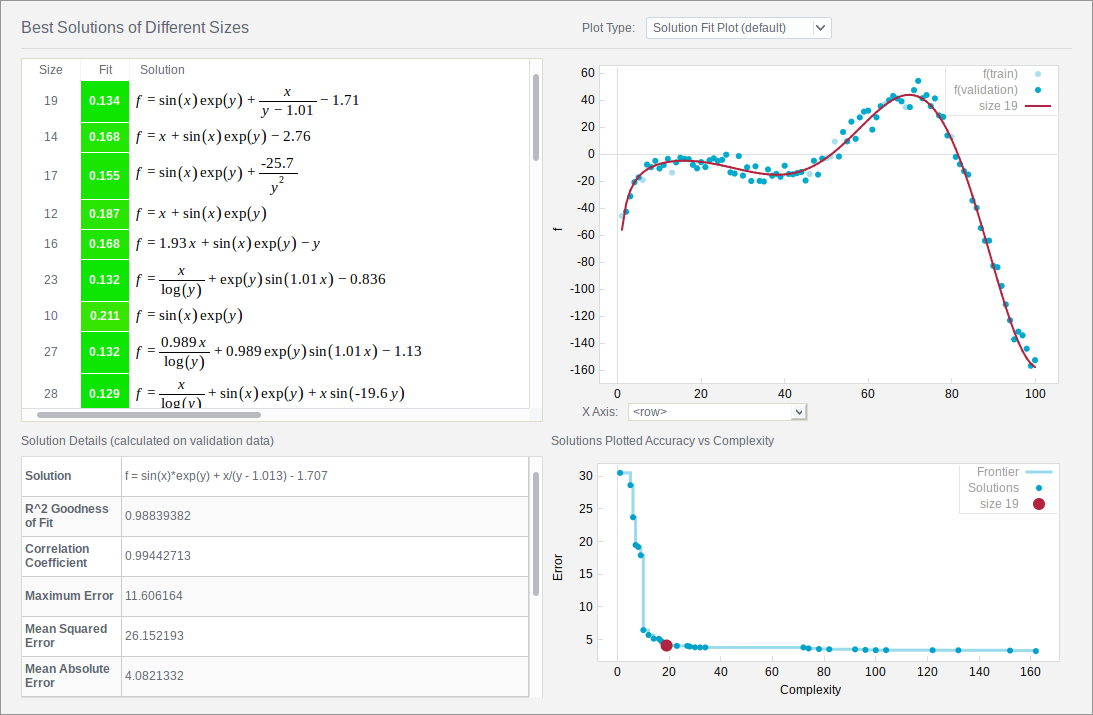
\includegraphics[width=\linewidth]{pics/sol_10perc.png}
        \caption{Run on the noisy function values with $\sigma = 5$}
        \label{fig:s_5}
    \end{figure}

    As Eureqa was able to find exact solutions for the noises, that can be found
    in real life, let's put it under really synthetic test. Let's add noise with
    $\sigma = 5$, which is 10\% of the std. This really messes the values
    (\autoref{fig:s_5}). But even though it was able to find almost the exact
    solution (6th solution on the \autoref{fig:s_5}), but did not choose it. The
    reason for this is the trade-off between complexity and error. It doesn't
    worth decreasing error by $0.002$ (6th solution's error is 0.132, while the
    error of the 1st solution is 0.134), while increasing the complexity by 4.
    Moreover, in favor of the 1st solution, it is possible to say (with some
    assumptions) that $y - 1 \approx \sin(y)$.

    \begin{figure}[H]
        \centering
        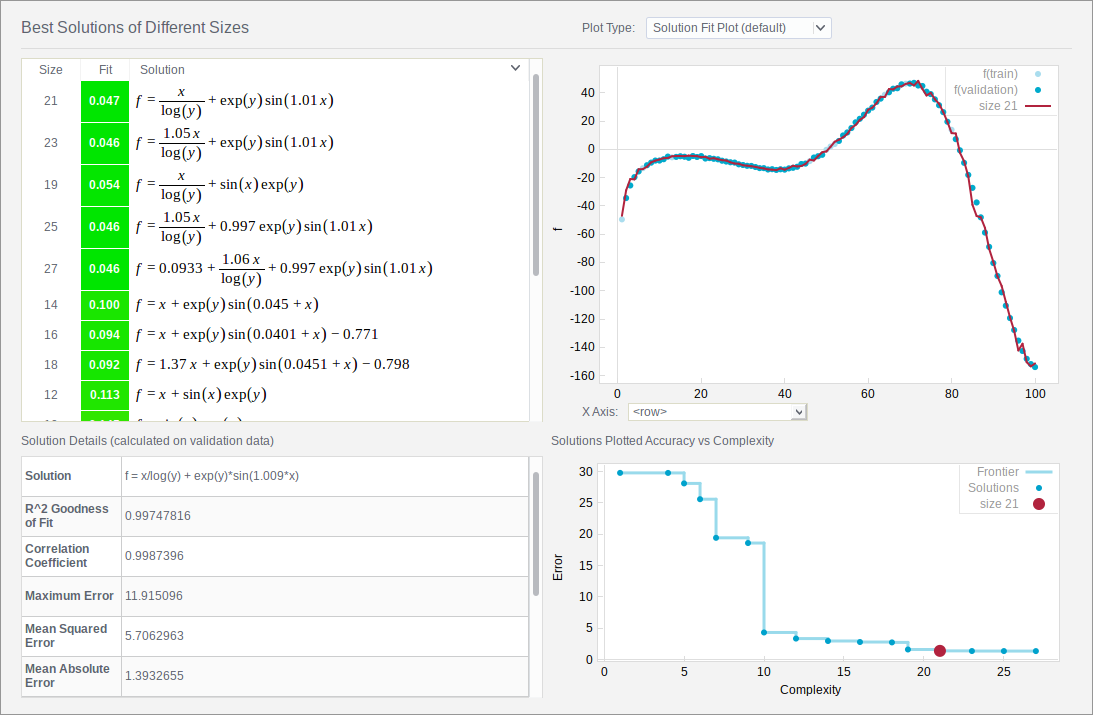
\includegraphics[width=\linewidth]{pics/sol_noisy.png}
        \caption{Run on the noisy data with $\sigma = 0.5$ for the function
            values and $\sigma_x = 0.05, \sigma_y = 0.02$ for the arguments}
        \label{fig:noisy}
    \end{figure}

    Before now we have tested on the data with noise only in function values.
    Now let's add noise to the arguments (which is more common in real life)
    and check how Eureqa will find the solution. For function values $\sigma$ is equal
    to $0.5$, which is 1\% of its std. For x and y arguments the $\sigma$ was
    chosen $0.05$ and $0.02$ respectively, which is 1\% of their stds each. As
    \autoref{fig:noisy} shows, the program was able to find the solution:
    $$f(x, y) = \frac{x}{\log(y)} - e^y\sin(1.009x)$$
    but it is not exact solution. Eureqa was even able to find the exact solution,
    but did not choose it as it decided that complexity difference of 2 doesn't
    worth error difference of 0.007 (which is relatively high). Anyway, we can
    see that Eureqa was able to find the exact form of the function and the first
    5 solutions are somehow similar.

\section{Conclusion}
    From the experiments (\autoref{sec:experiments}), it is obvious that GP
    implemented in Eureqa reconstructs our function pretty accurate. Whatever
    noise we add, Eureqa finds the function even if it is not the exact, but approximate
    solution. However, in general, it is unable to find every function accurately
    by the data generated. The complexity is the crucial parameter for GP. The more
    complex the function, the less it is able to find the solution.

    Returning to our experiment, the statistical significance of the experiments
    can be evaluated by $R^2$ values (R-squared is a statistical measure of how
    close the data are to the fitted regression line) given in the figures in
    \autoref{sec:experiments}. All the values are close to 1 and evaluated on
    the validation data. Thus our experiments are reliable.

    In Eureqa, correct solution for noise-free data lays on the line with the
    minimum error (which is 0 as it is noise-free). Here we don't even consider
    complexity as it finds the exact solution and stops evolving. On the
    noisy data, the program was balancing error and complexity, thus the solution
    was close to the ``knee'' of the front. However, being close, it choose
    whether it is reasonable to decrease complexity while increasing error or not.

    Thus, we can give the guide on choosing the most reliable (non-dominated)
    solution: it can be chosen by trading-off error vs. complexity. We should
    minimize both of them, but it is not always possible. We need to choose which
    parameter decreases most while increasing the other and think if it worth
    increasing it. The examples were given in the experiment (e.g. for
    \autoref{fig:s_5}: it doesn't worth decreasing error by $0.002$, while
    increasing the complexity by 4). However, we also need to remember that
    choosing more complex solutions can lead us to overfitting, thus sometimes
    we need to sacrifice error to avoid overfitting.

    Concluding, GP is very useful tool and can be applied to many areas of CS.
    For example, machine learning: what function describes our data, to predict
    new values for the new data (e.g. regression, time series, etc.). The real
    life example can be predicting the stocks of Google in short period of time
    in the future.

\end{document}
